\documentclass[12pt, a4paper]{article}

% ── Packages ──────────────────────────────────────────────────────────────────
\usepackage{amsmath, amssymb, amsthm}
\usepackage{geometry}
\usepackage{booktabs}
\usepackage{array}
\usepackage{hyperref}
\usepackage{xcolor}
\usepackage{tcolorbox}
\usepackage{enumitem}
\usepackage{parskip}
\usepackage{tikz}
\usetikzlibrary{arrows.meta, positioning, calc}

\geometry{margin=2.5cm}

% ══════════════════════════════════════════════════════════════════════════════
% ── Student-mode switch ───────────────────────────────────────────────────────
\newif\ifstudentmode
\studentmodefalse       % default: instructor mode

\ifx\studentflag\undefined
\else
  \studentmodetrue
\fi
% ══════════════════════════════════════════════════════════════════════════════

% ── Student-mode macros ───────────────────────────────────────────────────────
\newcommand{\sol}[2][6cm]{%
  \ifstudentmode
    \underline{\hspace{#1}}%
  \else
    {#2}%
  \fi
}

\newcommand{\soleq}[2][3cm]{%
  \ifstudentmode
    \par\vspace{4pt}%
    \noindent\rule{\linewidth}{0.5pt}\\[#1]%
    \noindent\rule{\linewidth}{0.5pt}%
    \par\vspace{4pt}%
  \else
    \[#2\]%
  \fi
}
% ──────────────────────────────────────────────────────────────────────────────

% ── Colors & boxes ────────────────────────────────────────────────────────────
\definecolor{mainblue}{RGB}{30, 100, 180}
\definecolor{boxbg}{RGB}{235, 243, 255}
\definecolor{notebg}{RGB}{255, 248, 230}
\definecolor{warnbg}{RGB}{255, 235, 235}

\tcbuselibrary{skins, breakable}

\newtcolorbox{resultbox}{
  colback=boxbg, colframe=mainblue,
  boxrule=1.2pt, arc=4pt,
  title={Result},
  fonttitle=\bfseries\color{white},
  coltitle=white, attach boxed title to top left={yshift=-2mm, xshift=4mm},
  boxed title style={colback=mainblue, arc=3pt}
}

\newtcolorbox{notebox}{
  colback=notebg, colframe=orange!70!black,
  boxrule=1pt, arc=4pt,
  left=4pt, right=4pt
}

\newtcolorbox{warnbox}{
  colback=warnbg, colframe=red!60!black,
  boxrule=1pt, arc=4pt,
  left=4pt, right=4pt
}

% ── Theorem environments ───────────────────────────────────────────────────────
\theoremstyle{definition}
\newtheorem{example}{Example}[section]

% ── Math macros ───────────────────────────────────────────────────────────────
\newcommand{\bth}{\boldsymbol{\theta}}
\newcommand{\bx}{\mathbf{x}}
\newcommand{\bX}{\mathbf{X}}
\newcommand{\by}{\mathbf{y}}
\newcommand{\bW}{\mathbf{W}}
\newcommand{\bb}{\mathbf{b}}
\newcommand{\bh}{\mathbf{h}}
\newcommand{\yhat}{\hat{y}}
\newcommand{\sigmoid}{\sigma}
\newcommand{\relu}{\mathrm{ReLU}}

% ── Document ──────────────────────────────────────────────────────────────────
\begin{document}

\begin{center}
  {\LARGE \textbf{Section 3.1: The XOR Problem}} \\[0.3em]
  {\large\itshape Why Linear Models Are Not Enough} \\[0.5em]
  {\large AI Class — Lecture Notes}%
  \ifstudentmode
    \quad {\normalsize\color{gray}[Student Copy]}%
  \fi
\end{center}

\vspace{1em}
\hrule
\vspace{1.5em}

% ══════════════════════════════════════════════════════════════════════════════
\section{The XOR Dataset}

The \textbf{exclusive OR} (XOR) function takes two binary inputs and outputs 1
if and only if \emph{exactly one} of them is 1:

\begin{center}
\renewcommand{\arraystretch}{1.2}
\begin{tabular}{ccc}
\toprule
$x_1$ & $x_2$ & $y$ \\
\midrule
0 & 0 & 0 \\
0 & 1 & 1 \\
1 & 0 & 1 \\
1 & 1 & 0 \\
\bottomrule
\end{tabular}
\end{center}

Notice that this is the same four input points used in the linear regression
example of Section~1.1, but the labels have changed: instead of $y = x_1 + x_2$
(a perfectly linear relationship), the output is now $y = x_1 \oplus x_2$
(XOR), which is \emph{non-linear}.

The question we will answer in this section is:
\textbf{Can a linear model learn XOR?} And if not — what can?

% ══════════════════════════════════════════════════════════════════════════════
\section{Linear Regression Fails on XOR}

Applying the normal equations $\bth = (\bX^{\top}\bX)^{-1}\bX^{\top}\by$ to
the XOR dataset:

\[
  \bX =
  \begin{bmatrix} 1 & 0 & 0 \\ 1 & 0 & 1 \\ 1 & 1 & 0 \\ 1 & 1 & 1 \end{bmatrix},
  \qquad
  \by =
  \begin{bmatrix} 0 \\ 1 \\ 1 \\ 0 \end{bmatrix}.
\]

Computing:
\[
  \bX^{\top}\bX =
  \begin{bmatrix} 4 & 2 & 2 \\ 2 & 2 & 1 \\ 2 & 1 & 2 \end{bmatrix},
  \qquad
  \bX^{\top}\by =
  \begin{bmatrix} 2 \\ 1 \\ 1 \end{bmatrix}.
\]

Solving $(\bX^{\top}\bX)\,\bth = \bX^{\top}\by$ gives:

% ── \sol applied: student solves the system ──────────────────────────────────
\soleq[2.5cm]{%
  \bth =
  \begin{bmatrix} b \\ w_1 \\ w_2 \end{bmatrix}
  =
  \begin{bmatrix} 0.5 \\ 0 \\ 0 \end{bmatrix}
}
% ─────────────────────────────────────────────────────────────────────────────

The model predicts $\yhat = 0.5$ for \emph{every} input, regardless of $x_1$
and $x_2$.  The resulting MSE is:

\[
  \mathrm{MSE}
  = \frac{(0.5)^2 + (-0.5)^2 + (-0.5)^2 + (0.5)^2}{4}
  = \sol[4cm]{0.25}.
\]

\begin{warnbox}
\textbf{This is the best any linear regression model can do on XOR.}
No choice of $w_1, w_2, b$ can reduce the MSE below $0.25$ — not because
the model is poorly tuned, but because the relationship is fundamentally
non-linear.
\end{warnbox}

% ══════════════════════════════════════════════════════════════════════════════
\section{Logistic Regression Also Fails}

Logistic regression tries to separate the two classes with a \textbf{linear
decision boundary}: the line $w_1 x_1 + w_2 x_2 + b = 0$.

\begin{center}
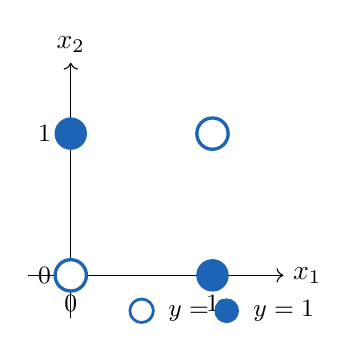
\begin{tikzpicture}[scale=1.8]
  % Axes
  \draw[->] (-0.3, 0) -- (1.5, 0) node[right] {$x_1$};
  \draw[->] (0, -0.3) -- (0, 1.5) node[above] {$x_2$};
  \foreach \x in {0,1} \draw (\x, 2pt) -- (\x, -2pt) node[below] {\small\x};
  \foreach \y in {0,1} \draw (2pt, \y) -- (-2pt, \y) node[left]  {\small\y};

  % y=0 points (circles)
  \node[draw=mainblue, fill=white, circle, inner sep=4pt, line width=1.2pt]
    at (0,0) {};
  \node[draw=mainblue, fill=white, circle, inner sep=4pt, line width=1.2pt]
    at (1,1) {};
  % y=1 points (filled)
  \node[draw=mainblue, fill=mainblue, circle, inner sep=4pt]
    at (0,1) {};
  \node[draw=mainblue, fill=mainblue, circle, inner sep=4pt]
    at (1,0) {};

  % Legend
  \node[draw=mainblue, fill=white, circle, inner sep=3pt, line width=1pt]
    at (0.5, -0.25) {};
  \node[anchor=west] at (0.62,-0.25) {\small $y=0$};
  \node[draw=mainblue, fill=mainblue, circle, inner sep=3pt]
    at (1.1, -0.25) {};
  \node[anchor=west] at (1.22,-0.25) {\small $y=1$};
\end{tikzpicture}
\end{center}

The two classes are arranged in a \textbf{checkerboard pattern}: no single
straight line can put all the filled dots on one side and all the open dots
on the other.

\begin{resultbox}
XOR is \textbf{not linearly separable}.  Any linear classifier — whether
linear regression or logistic regression — will produce a decision boundary
that misclassifies at least two of the four points.
The best logistic regression can do is predict $\hat{p} = 0.5$ everywhere
(cross-entropy loss $= \ln 2 \approx 0.693$ per sample).
\end{resultbox}

% ══════════════════════════════════════════════════════════════════════════════
\section{The Key Insight: Feature Transformation}

What if, instead of feeding $(x_1, x_2)$ directly to a linear classifier,
we first \textbf{transform} the inputs into a new space where XOR
\emph{is} linearly separable?

Define two new features:
\begin{align*}
  h_1 &= \text{step}(x_1 + x_2 - 0.5)
         \quad\text{(detects: at least one input is 1)} \\
  h_2 &= \text{step}(x_1 + x_2 - 1.5)
         \quad\text{(detects: both inputs are 1)}
\end{align*}

where $\text{step}(z) = 1$ if $z \ge 0$, else $0$.  Computing these for all
four inputs:

\begin{center}
\renewcommand{\arraystretch}{1.2}
\begin{tabular}{cc|cc|c}
\toprule
$x_1$ & $x_2$ & $h_1$ & $h_2$ & $y$ \\
\midrule
0 & 0 & 0 & 0 & 0 \\
0 & 1 & 1 & 0 & 1 \\
1 & 0 & 1 & 0 & 1 \\
1 & 1 & 1 & 1 & 0 \\
\bottomrule
\end{tabular}
\end{center}

In the new feature space $(h_1, h_2)$ we need to output 1 when $(h_1, h_2)
= (1, 0)$ and 0 otherwise.  This \emph{is} linearly separable:
\[
  y = h_1 - h_2.
\]

\begin{notebox}
\textbf{Insight.}
The hidden features $h_1$ and $h_2$ compute an OR gate and an AND gate,
respectively.  XOR is OR minus AND.  The non-linear step function in each
neuron is what makes the new representation useful — a purely linear
transformation of $(x_1, x_2)$ cannot produce a linearly separable space
for XOR.
\end{notebox}

% ══════════════════════════════════════════════════════════════════════════════
\section{A Feedforward Neural Network}

The transformation above has a natural network structure:

\begin{center}
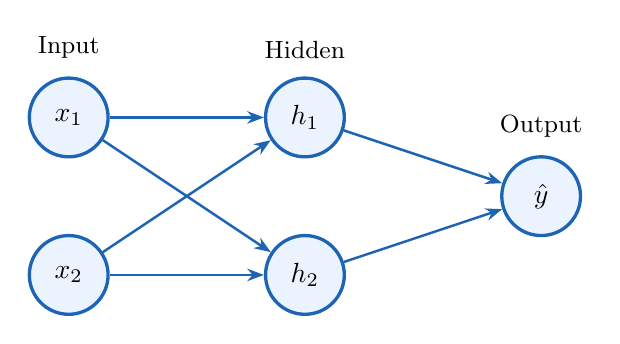
\begin{tikzpicture}[
    neuron/.style={circle, draw=mainblue, fill=boxbg,
                   minimum size=1cm, line width=1.2pt},
    arr/.style={-{Stealth[length=6pt]}, mainblue, line width=0.9pt},
    lbl/.style={font=\small}
  ]

  % Input layer
  \node[neuron] (x1) at (0, 1)  {$x_1$};
  \node[neuron] (x2) at (0,-1)  {$x_2$};
  \node[above=0.1cm of x1, lbl] {Input};

  % Hidden layer
  \node[neuron] (h1) at (3, 1)  {$h_1$};
  \node[neuron] (h2) at (3,-1)  {$h_2$};
  \node[above=0.1cm of h1, lbl] {Hidden};

  % Output layer
  \node[neuron] (y)  at (6, 0)  {$\yhat$};
  \node[above=0.1cm of y,  lbl] {Output};

  % Edges: input → hidden
  \draw[arr] (x1) -- (h1);
  \draw[arr] (x1) -- (h2);
  \draw[arr] (x2) -- (h1);
  \draw[arr] (x2) -- (h2);

  % Edges: hidden → output
  \draw[arr] (h1) -- (y);
  \draw[arr] (h2) -- (y);

\end{tikzpicture}
\end{center}

\subsection{Forward Pass}

Let $g$ denote the hidden activation function (e.g.\ step, sigmoid, or ReLU).
The computation proceeds in two steps:

\textbf{Hidden layer} — apply a linear transformation, then a non-linearity:

\begin{equation}
  \bh = g\!\left(\bW^{(1)}\bx + \bb^{(1)}\right),
  \label{eq:hidden}
\end{equation}

where $\bW^{(1)} \in \mathbb{R}^{2 \times 2}$ and $\bb^{(1)} \in \mathbb{R}^2$
are the weights and biases of the hidden layer.

\textbf{Output layer} — a linear combination of the hidden features:

\begin{equation}
  \yhat = \bW^{(2)}\bh + b^{(2)}.
  \label{eq:output}
\end{equation}

\subsection{Weights That Solve XOR}

The construction in Section~4 corresponds to the following network parameters:

\[
  \bW^{(1)} =
  \begin{bmatrix} 1 & 1 \\ 1 & 1 \end{bmatrix},
  \quad
  \bb^{(1)} =
  \begin{bmatrix} -0.5 \\ -1.5 \end{bmatrix},
  \quad
  \bW^{(2)} =
  \begin{bmatrix} 1 & -1 \end{bmatrix},
  \quad
  b^{(2)} = 0.
\]

Verify for the input $(x_1, x_2) = (1, 1)$:

\[
  \bh
  = \text{step}\!\left(
      \begin{bmatrix}1&1\\1&1\end{bmatrix}
      \begin{bmatrix}1\\1\end{bmatrix}
      +
      \begin{bmatrix}-0.5\\-1.5\end{bmatrix}
    \right)
  = \text{step}\!\left(\begin{bmatrix}1.5\\0.5\end{bmatrix}\right)
  = \sol[3cm]{\begin{bmatrix}1\\1\end{bmatrix}},
\]

\[
  \yhat
  = \begin{bmatrix}1 & -1\end{bmatrix}
    \begin{bmatrix}1\\1\end{bmatrix}
  = \sol[3cm]{0}. \quad\checkmark
\]

% ══════════════════════════════════════════════════════════════════════════════
\section{From Hand-Crafted to Learned Features}

The weights above were designed by hand.  In practice, with high-dimensional
data and complex patterns, we cannot design features manually.

The power of a neural network is that the \textbf{weights are learned from
data} using gradient descent on a suitable loss function.  The network
discovers which hidden features are useful, automatically.

\begin{notebox}
\textbf{Why depth matters.}
A network with \emph{no} hidden layer is just a linear model.  Adding even
\emph{one} hidden layer with a non-linear activation turns the network into a
\textbf{universal function approximator}: given enough neurons, it can
approximate any continuous function to arbitrary precision (Universal
Approximation Theorem).
\end{notebox}

% ══════════════════════════════════════════════════════════════════════════════
\section{Summary}

\begin{center}
\renewcommand{\arraystretch}{1.5}
\begin{tabular}{ll}
\toprule
\textbf{Problem}          & XOR is not linearly separable \\
\textbf{Linear models}    & Both linear and logistic regression predict a constant \\
\textbf{Fix}              & Add a hidden layer with a non-linear activation \\
\textbf{Key idea}         & Hidden neurons learn a new feature space where the \\
                          & task is linearly separable \\
\textbf{Forward pass}     & $\bh = g(\bW^{(1)}\bx + \bb^{(1)})$,\;
                            $\yhat = \bW^{(2)}\bh + b^{(2)}$ \\
\bottomrule
\end{tabular}
\end{center}

\bigskip
\textbf{Up next (Section~3.2):} How do we \emph{train} a feedforward network?
We need to compute gradients of the loss with respect to every weight in the
network — this is the \textbf{backpropagation} algorithm.

\end{document}
